\documentclass[a4paper,12pt,oneside]{book}

%-------------------------------Start of the Preable------------------------------------------------
\usepackage[english]{babel}
\usepackage{blindtext}
%packagr for hyperlinks
\usepackage{hyperref}
\hypersetup{
    colorlinks=true,
    linkcolor=blue,
    filecolor=magenta,      
    urlcolor=cyan,
}

\urlstyle{same}
%use of package fancy header
\usepackage{fancyhdr}
\setlength\headheight{26pt}
\fancyhf{}
%\rhead{
\includegraphics[width=1cm]{logo}}
\lhead{\rightmark}
\rhead{
\includegraphics[width=1cm]{logo}}
\fancyfoot[RE, RO]{\thepage}
\fancyfoot[CE, CO]{\href{http://www.e-yantra.org}{www.e-yantra.org}}

\pagestyle{fancy}

%use of package for section title formatting
\usepackage{titlesec}
\titleformat{\chapter}
  {\Large\bfseries} % format
  {}                % label
  {0pt}             % sep
  {\huge}           % before-code
 
%use of package tcolorbox for colorful textbox
\usepackage[most]{tcolorbox}
\tcbset{colback=cyan!5!white,colframe=cyan!75!black,halign title = flush center}

\newtcolorbox{mybox}[1]{colback=cyan!5!white,
colframe=cyan!75!black,fonttitle=\bfseries,
title=\textbf{\Large{#1}}}

%use of package marginnote for notes in margin
\usepackage{marginnote}
\usepackage{tabularx}
%use of packgage watermark for pages
%\usepackage{draftwatermark}
%\SetWatermarkText{
\includegraphics{logo}}
\usepackage[scale=2,opacity=0.1,angle=0]{background}
\backgroundsetup{
contents={
\includegraphics{logo}}
}

%use of newcommand for keywords color
\usepackage{xcolor}
\newcommand{\keyword}[1]{\textcolor{red}{\textbf{#1}}}

%package for inserting pictures
\usepackage{graphicx}

%package for highlighting
\usepackage{color,soul}

%new command for table
\newcommand{\head}[1]{\textnormal{\textbf{#1}}}


%----------------------End of the Preamble---------------------------------------


\begin{document}

%---------------------Title Page------------------------------------------------
\begin{titlepage}
\raggedright
{\Large eYSIP2017\\[1cm]}
{\Huge\scshape\centering Distributed robotics - multi swarm robots \\[.1in]}
\vfill
\hfill\\
\begin{figure}[h!]
	\centering\includegraphics[width=350px]{./Small_bots.jpg}		
\end{figure}	
\hfill\\
\begin{flushright}
{\large Intern 1 Mr. Chinmay C \\}
{\large Intern 2 Mr. R Hariharan \\}
{\large Mentor 1 Ms. Rutuja \\}
{\large Mentor 2 Ms. Deepa \\}
{\large Duration of Internship: $ 22/05/2017-07/07/2017 $ \\}
\end{flushright}

{\itshape 2017, e-Yantra Publication}
\end{titlepage}
%-------------------------------------------------------------------------------

\tableofcontents

\chapter[Distributed robotics - multi swarm robots Hardware manual]{Distributed robotics - multi swarm robots Hardware manual}
\section{Abstract}
Swarm robotics is a field in robotics which implements coordination of multi robot systems which consist of large number of robots having simpler robots. There is a collective behavior that emerges from interactions between robots and interactions of robots with the environment. This behavior is emerged from field of biological studies of fishes, birds, ants, insects, etc. Application of swarm robotics varies from military, aviation to collective behavior of self driving cars. The objective of the project was to build miniaturized swarm bots and develop an algorithm for generic shape formation.

\subsection*{Following points are completed:}
\begin{itemize}
\item Study the concepts of swarm robotics and get familiar
with different robots available 
\item Study the kinematics of differential drive configuration 
\item Selecting appropriate sensors to be added 
\item Designing the PCB 
\item Assembling all the components 
\item Making of Mini bots 
\item Testing of Mini bots
\item Implementing circle formation of asynchronous fat robots with limited visibility in V-REP simulator
\item Developing and implementing generic shape formation algorithm for a system of distributed robots in V-REP simulator
\item Implementing follow the leader swarm behavior on Mini bots
\item Implementing rendezvous swarm behavior on Firebird V robots
\end{itemize}

\chapter[Hardware parts]{Hardware parts}
\begin{itemize}
  \item List of all hardware components are available \href{./COMPONENT LIST/Small_robot_PCB_schematic_WITH_COST.pdf}{here} 
  \item Microcontroller Atmega16 \href{./datasheet/atmega16.pdf}{Datasheet}, {Chip component, Lamington road, Mumbai} 
  \item Hex buffer CD40106 \href{./datasheet/CD40106.pdf}{Datasheet}, {Chip component, Lamington road, Mumbai} 
  \item Motor driver L293D \href{./datasheet/L293.pdf}{Datasheet}, {GALA Electronics, Lamington road, Mumbai} 
  \item Comparator LM158 \href{./datasheet/lm158-n.pdf}{Datasheet}, {Chip component, Lamington road, Mumbai}
  \item Actuators BO motors: 60 rpm 12 volts	
  \item LCD 16x2: GALA Electronics, Lamington road, Mumbai
  \item Position encoders MOC7811: GALA Electronics, Lamington road, Mumbai
  \item ISP programmer STK500v2: \href{}, {Nex robotics}
  \item IR proximity sensors: GALA Electronics, Lamington road, Mumbai
\end{itemize}


\chapter[Softwares used]{Softwares used}
\begin{itemize}
	\item \textbf{Autodesk Eagle 7.6.0}
	\begin{itemize}
		\item \href{https://www.autodesk.com/products/eagle/overview}{Download Eagle}
		\item \href{https://www.youtube.com/user/EAGLECadSoftComputer}{Video tutorials on YouTube}
	\end{itemize}
  \item \textbf{V-rep 3.4.0}
  \begin{itemize}
  	\item \href{https://github.com/eYSIP-2017/eYSIP-2017_DistributedRobotics/blob/master/Documents/Manuals/Understanding_V_REP.pdf}{Understanding V-REP} for beginners
  	\item  \href{http://www.coppeliarobotics.com/downloads.html}{Downloading V-REP}
	\item  \href{http://www.coppeliarobotics.com/resources.html}{For more details on V-REP}
  \end{itemize}
  \item \textbf{Autodesk Fusion 360}
\begin{itemize}
	\item \href{https://www.autodesk.com/products/fusion-360/students-teachers-educators}{To download fusion 360 and get details on it}
\end{itemize}
  \item \textbf{Avrdude}
  \begin{itemize}
  	\item \href{http://www.nongnu.org/avrdude/}{To download Avrdude and get details on it}
  \end{itemize}
\item \textbf{Avrgcc}
 \begin{itemize}
 	\item Worked on windows platform
	\item \href{https://sourceforge.net/projects/winavr/files/}{To download Winavr to get avrgcc}
	\item \href{https://gcc.gnu.org/wiki/avr-gcc}{To understand avrgcc}
\end{itemize}
\item \textbf{Texstudio}
\begin{itemize}
	\item \href{http://www.texstudio.org/}{Download Texstudio}
\end{itemize}
\item \textbf{Git}
\begin{itemize}
	\item \href{https://github.com/eYSIP-2017/eYSIP-2017_DistributedRobotics.git}{Link} to our github repository
	\item \href{https://git-scm.com/}{Download Git}
\end{itemize}
\end{itemize}

\newpage

\chapter{Assembly of hardware}
Refer to our \href{https://github.com/eYSIP-2017/eYSIP-2017_DistributedRobotics/blob/master/Documents/Manuals/Hardware%20Manual/document.pdf}{Hardware Manual} to understand Mini Bot better
\section{Circuit Diagram}
\begin{figure}[h!]
	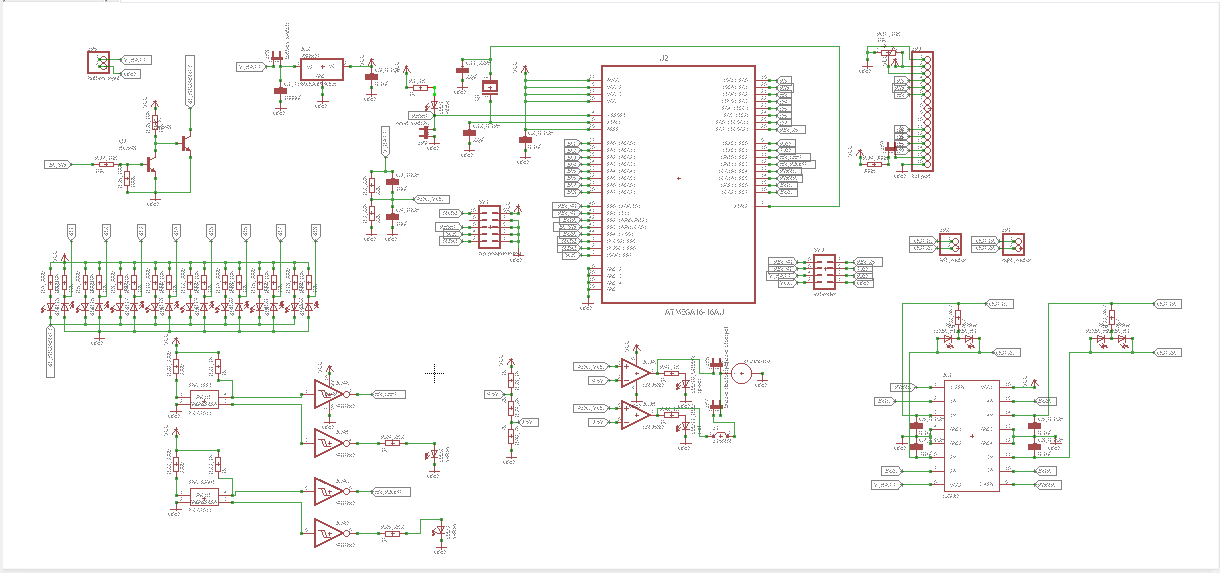
\includegraphics[width=\textwidth]{./PCB_schematic.png}		
	\caption{Overall schematic of Mini Bot PCB}
\end{figure}
\textbf{Main circuits:}	
\begin{itemize}
	\item L293D motor driver circuits: refer to Motion control section of \href{https://github.com/eYSIP-2017/eYSIP-2017_DistributedRobotics/blob/master/Documents/Manuals/Hardware%20Manual/document.pdf}{Hardware Manual}
	\item Position encoders circuits: refer to Position encoders section of \href{https://github.com/eYSIP-2017/eYSIP-2017_DistributedRobotics/blob/master/Documents/Manuals/Hardware%20Manual/document.pdf}{Hardware Manual}
	\item IR sensors circuits: refer to Infrared proximity and Directional
	light intensity sensors section of \href{https://github.com/eYSIP-2017/eYSIP-2017_DistributedRobotics/blob/master/Documents/Manuals/Hardware%20Manual/document.pdf}{Hardware Manual}
	\item Battery voltage sensor circuits: refer to Battery voltage sensor section of \href{https://github.com/eYSIP-2017/eYSIP-2017_DistributedRobotics/blob/master/Documents/Manuals/Hardware%20Manual/document.pdf}{Hardware Manual}
\end{itemize}
\section{Steps to build Mini Bots}
\subsection*{Step 1: PCB designing and routing}
\begin{figure}[h!]
	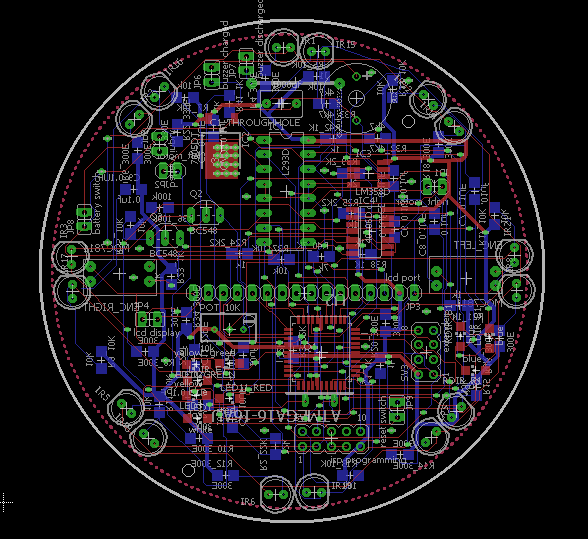
\includegraphics[width=0.5\textwidth]{./PCB_layout}
	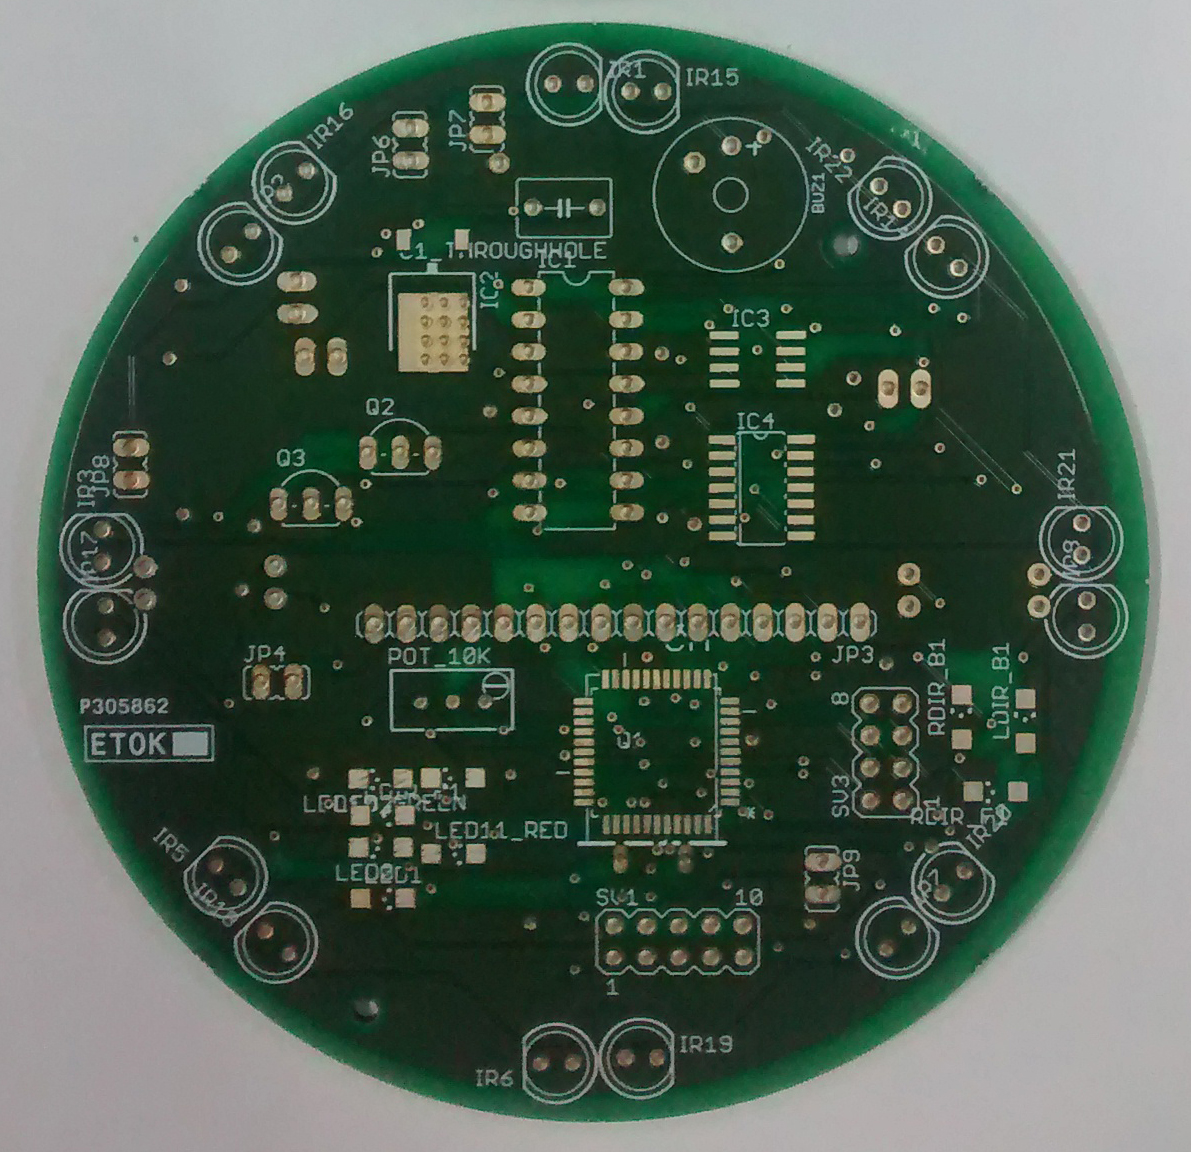
\includegraphics[width=0.47\textwidth]{./Pictures/PCB_front}		
	\caption{Routed and Printed PCB respectively}
\end{figure}	
We used Eagle software for designing the PCB. Gave printing of PCB to PCB power, Circuit Systems India Ltd., Gujarat.
\subsection*{Step 2: Designing of chassis}
We design chassis in Fusion 360 and got it laser cut on 5mm acrylic sheet in Tata Centre, IIT-B. The straight BO motors were fixed with L-clamps and then attached to chassis as shown in figure 4.3. 
\begin{figure}[h!]
	\centering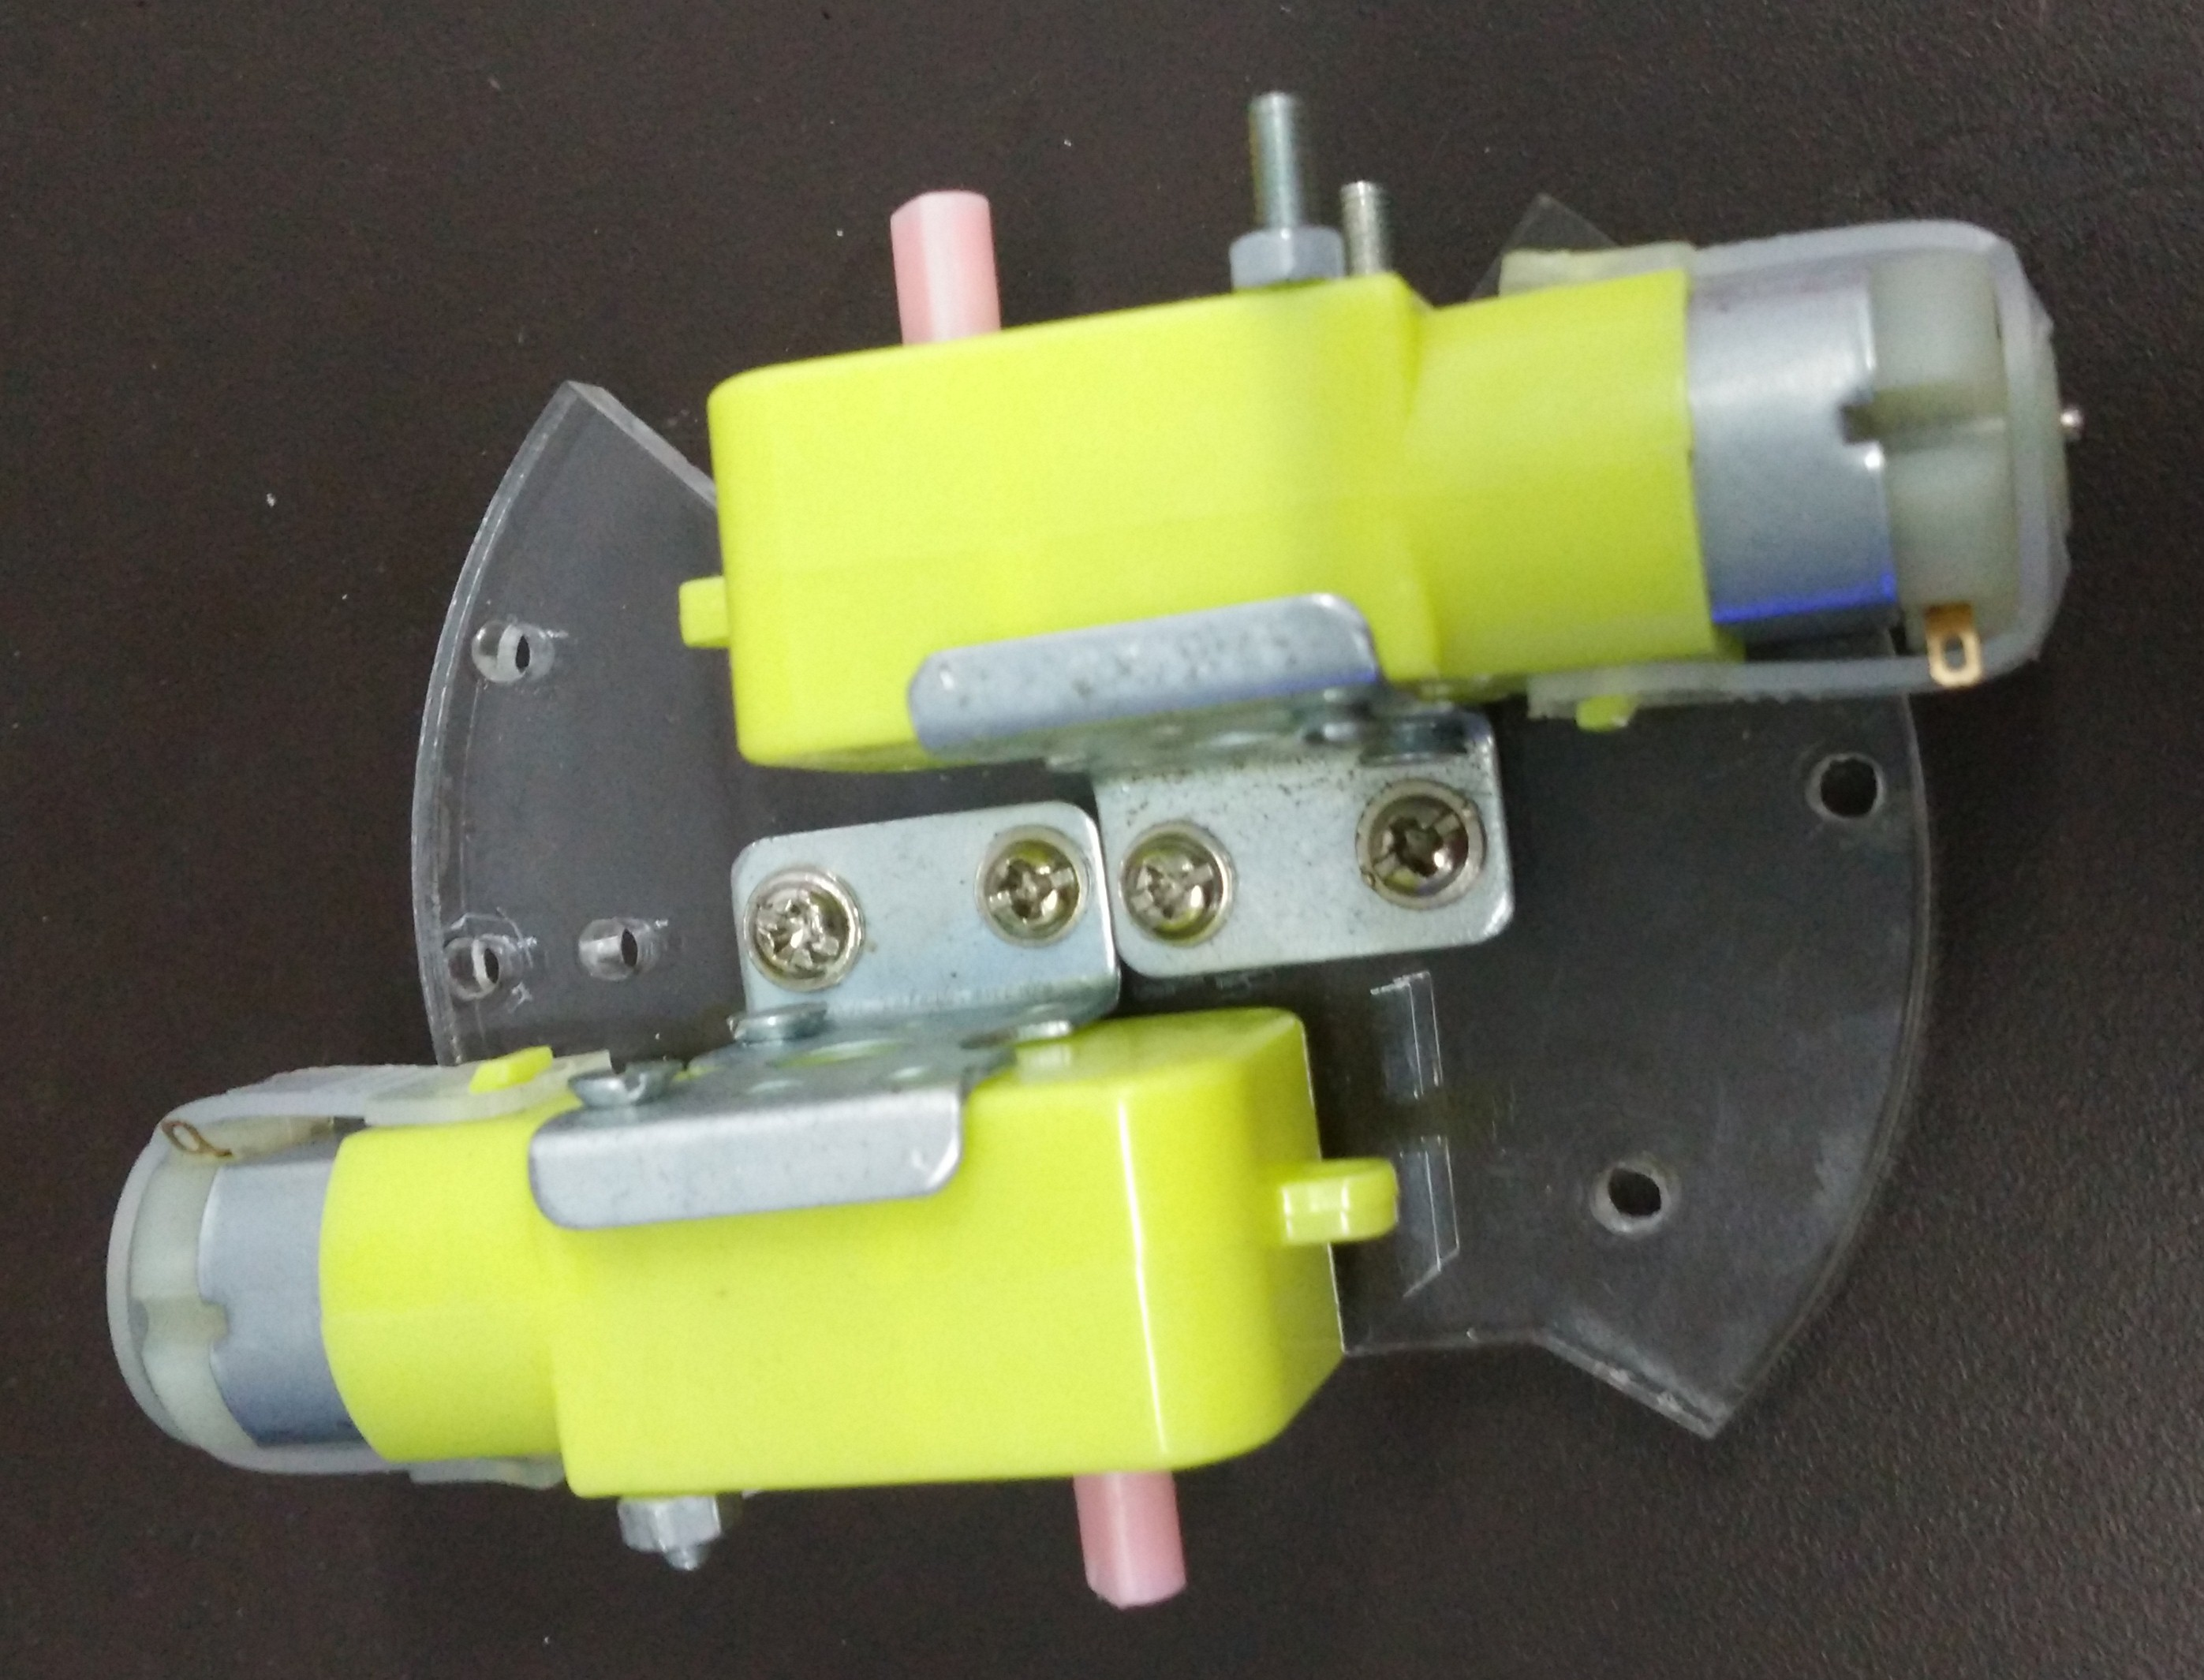
\includegraphics[width=180px]{./Pictures/Chassis_Design}		
	\caption{Chassis design}
\end{figure}	
       
\subsection*{Step 3: Soldering components on PCB}
Soldering the SMD components onto the PCB, based on the schematics.
\begin{figure}[h!]
	\centering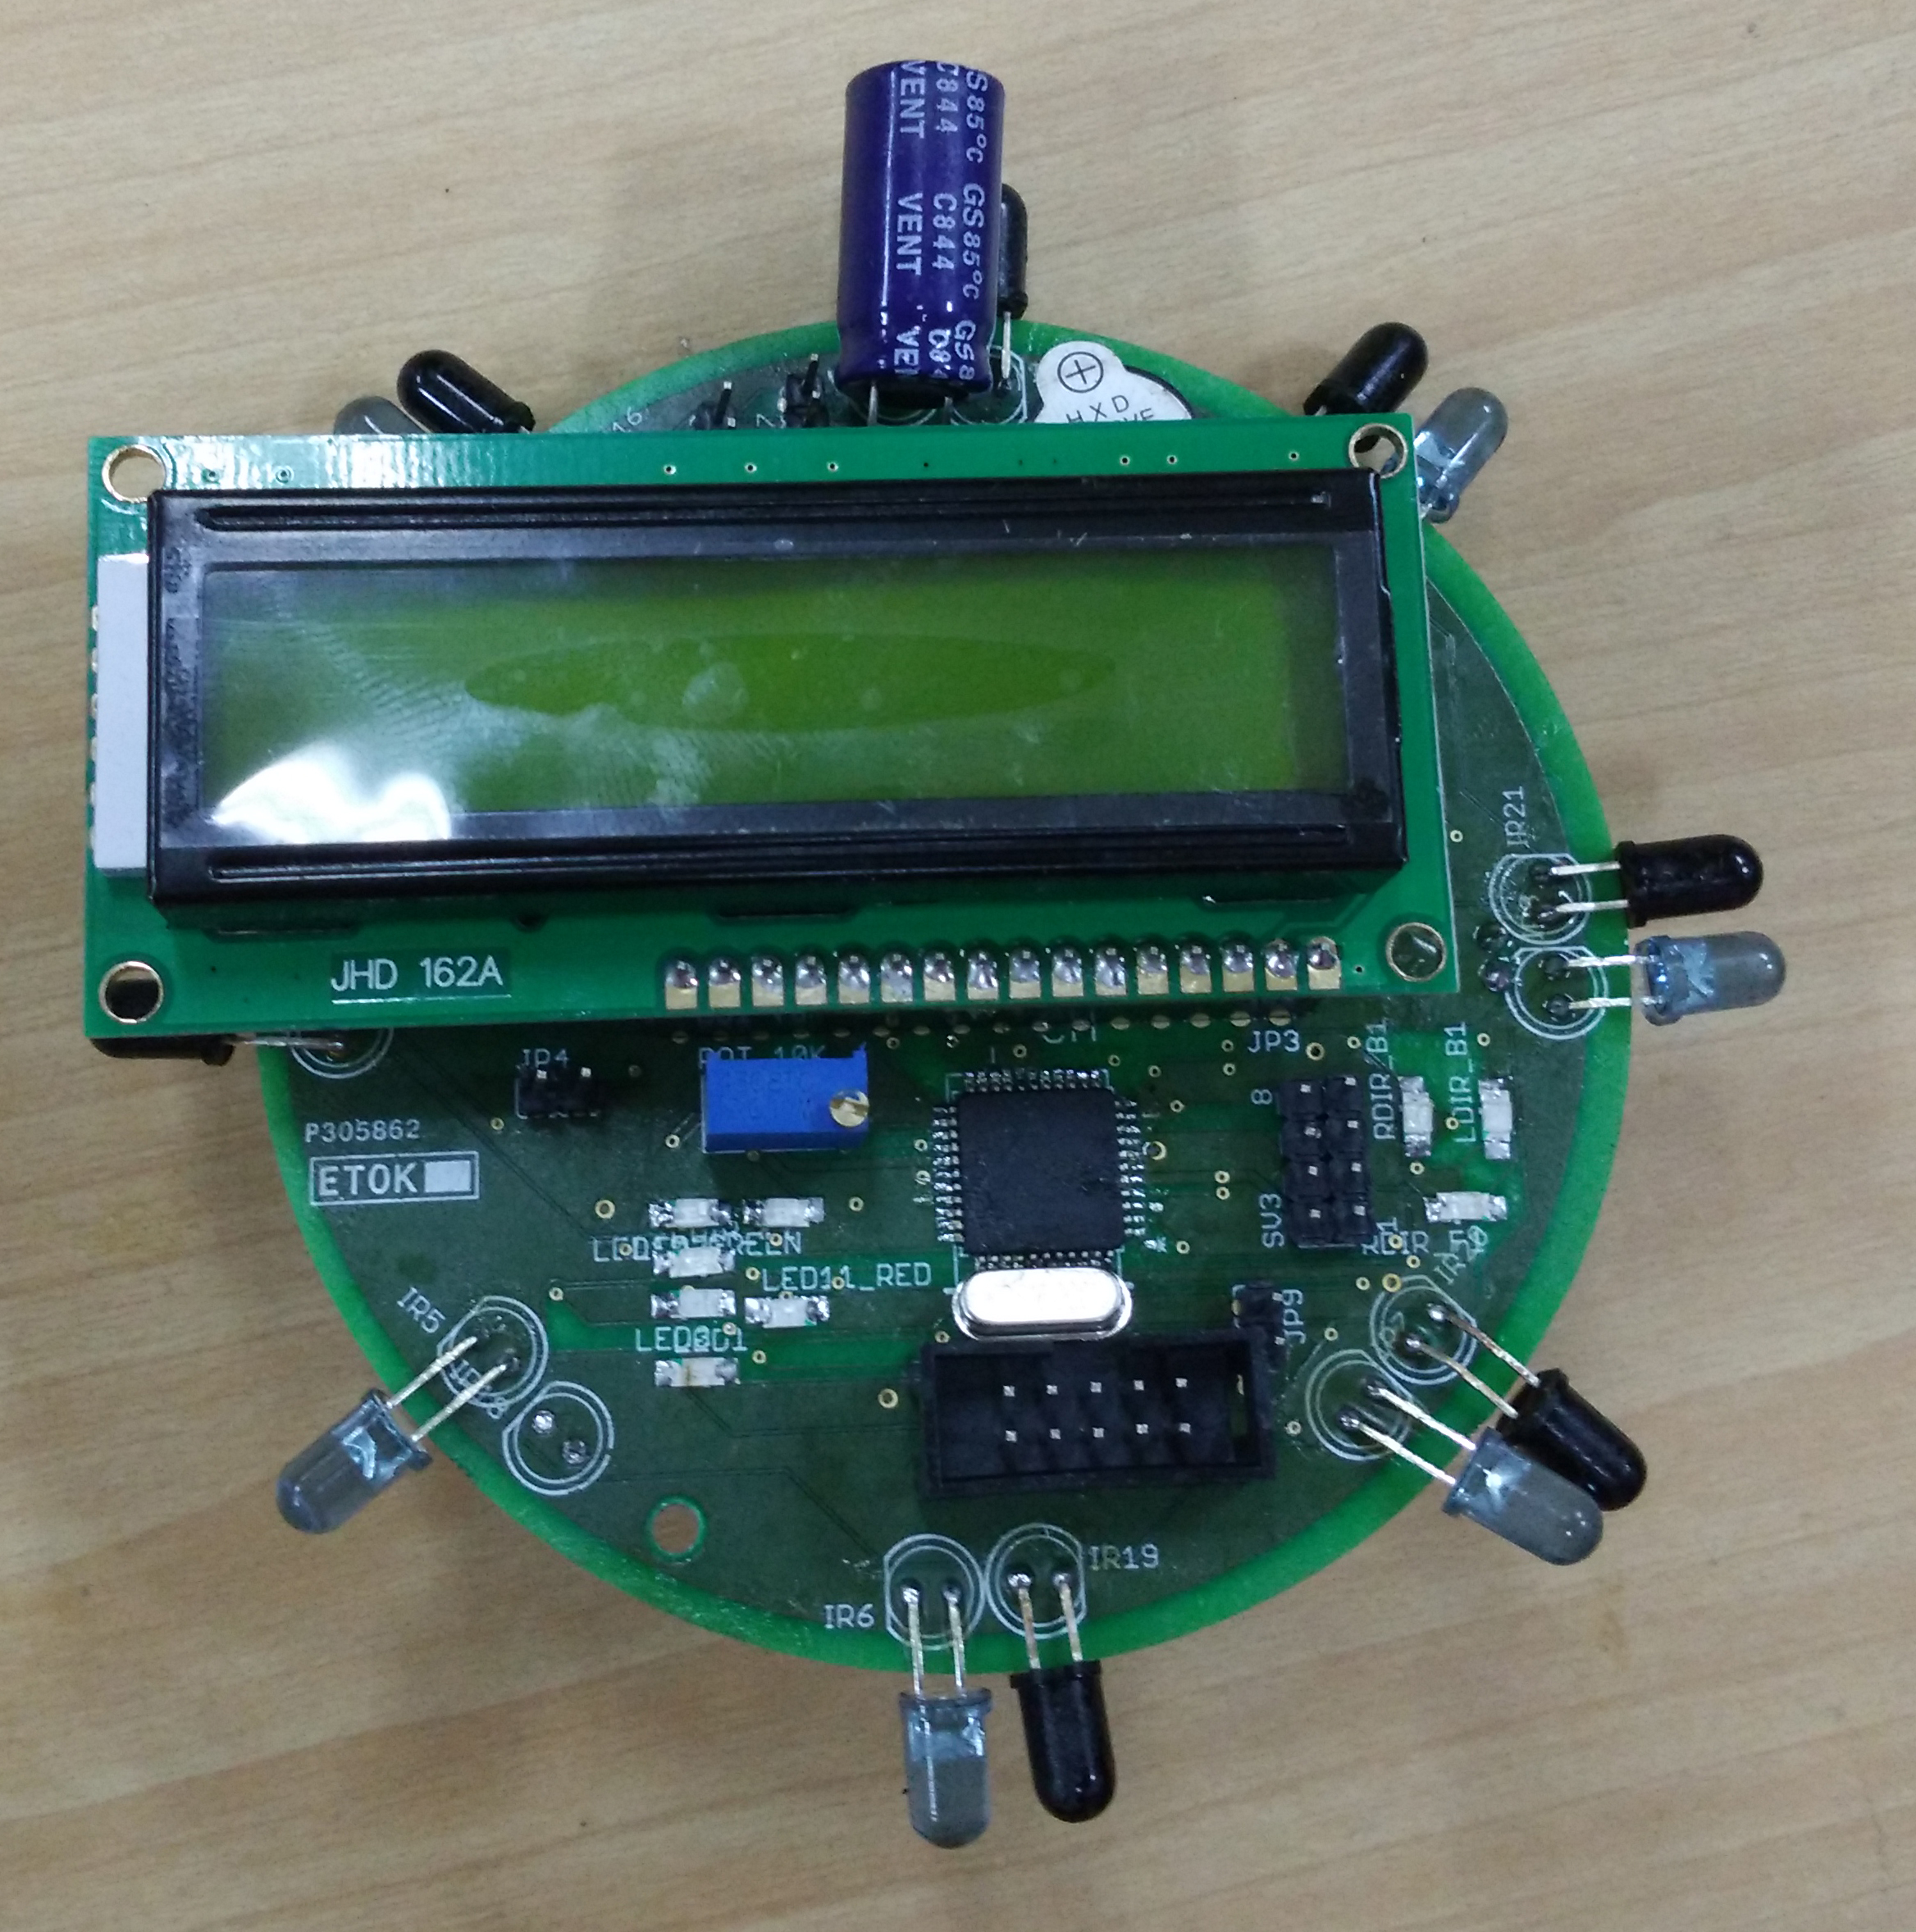
\includegraphics[width=0.6\textwidth]{./Pictures/PCB_interfaced_with_LCD}
	\caption{Soldered PCB}		
\end{figure}
\subsection*{Step 4: Assembling the robot}
The motors are attached to the chassis and the PCB is screwed to the chassis. The battery connections are appropriately made.
\begin{figure}[h!]
	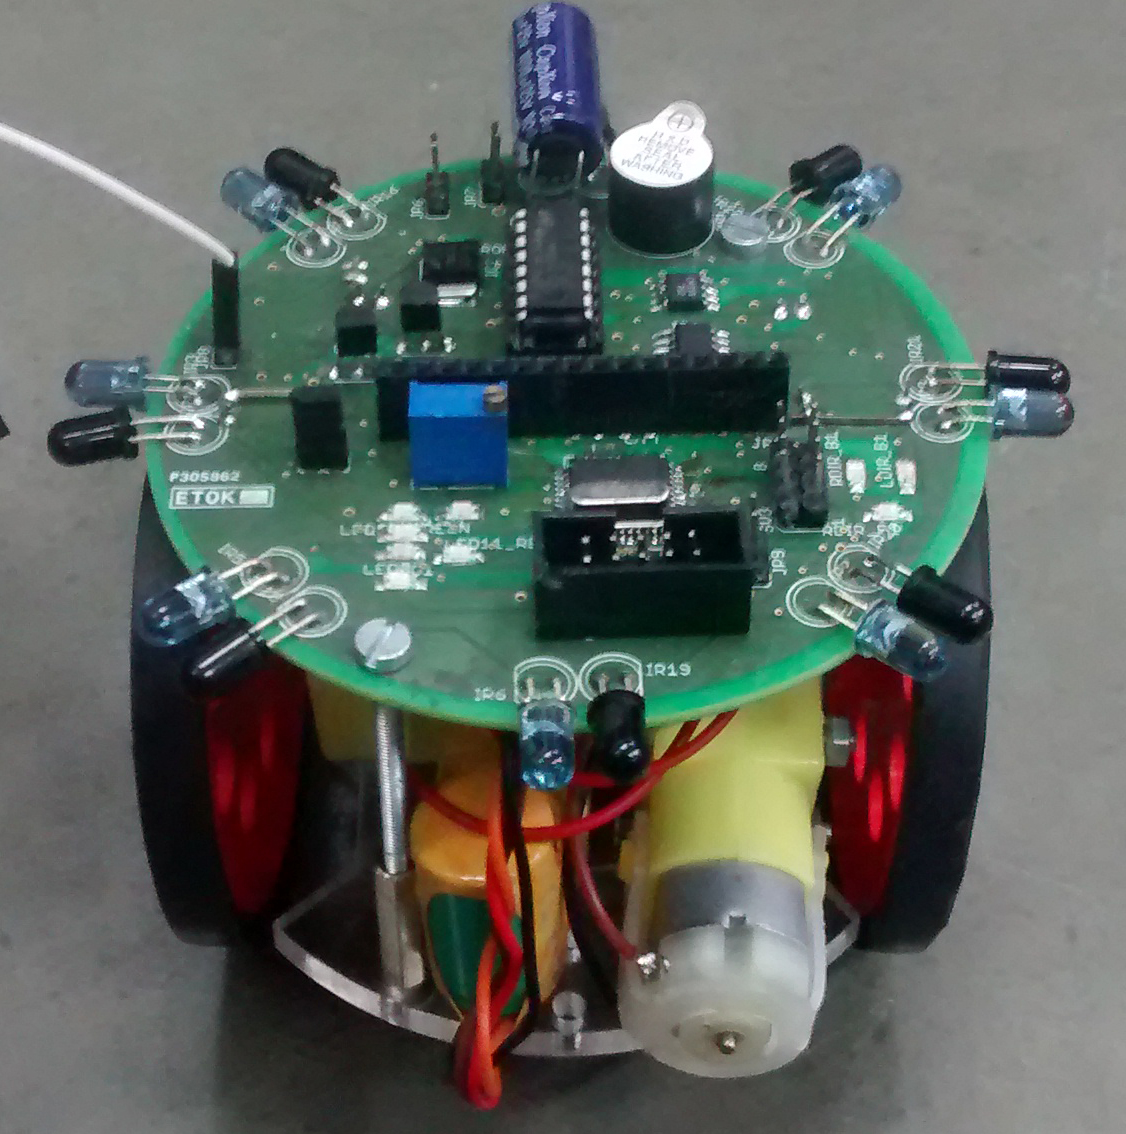
\includegraphics[width=0.30\textwidth]{./Pictures/version2_top}
	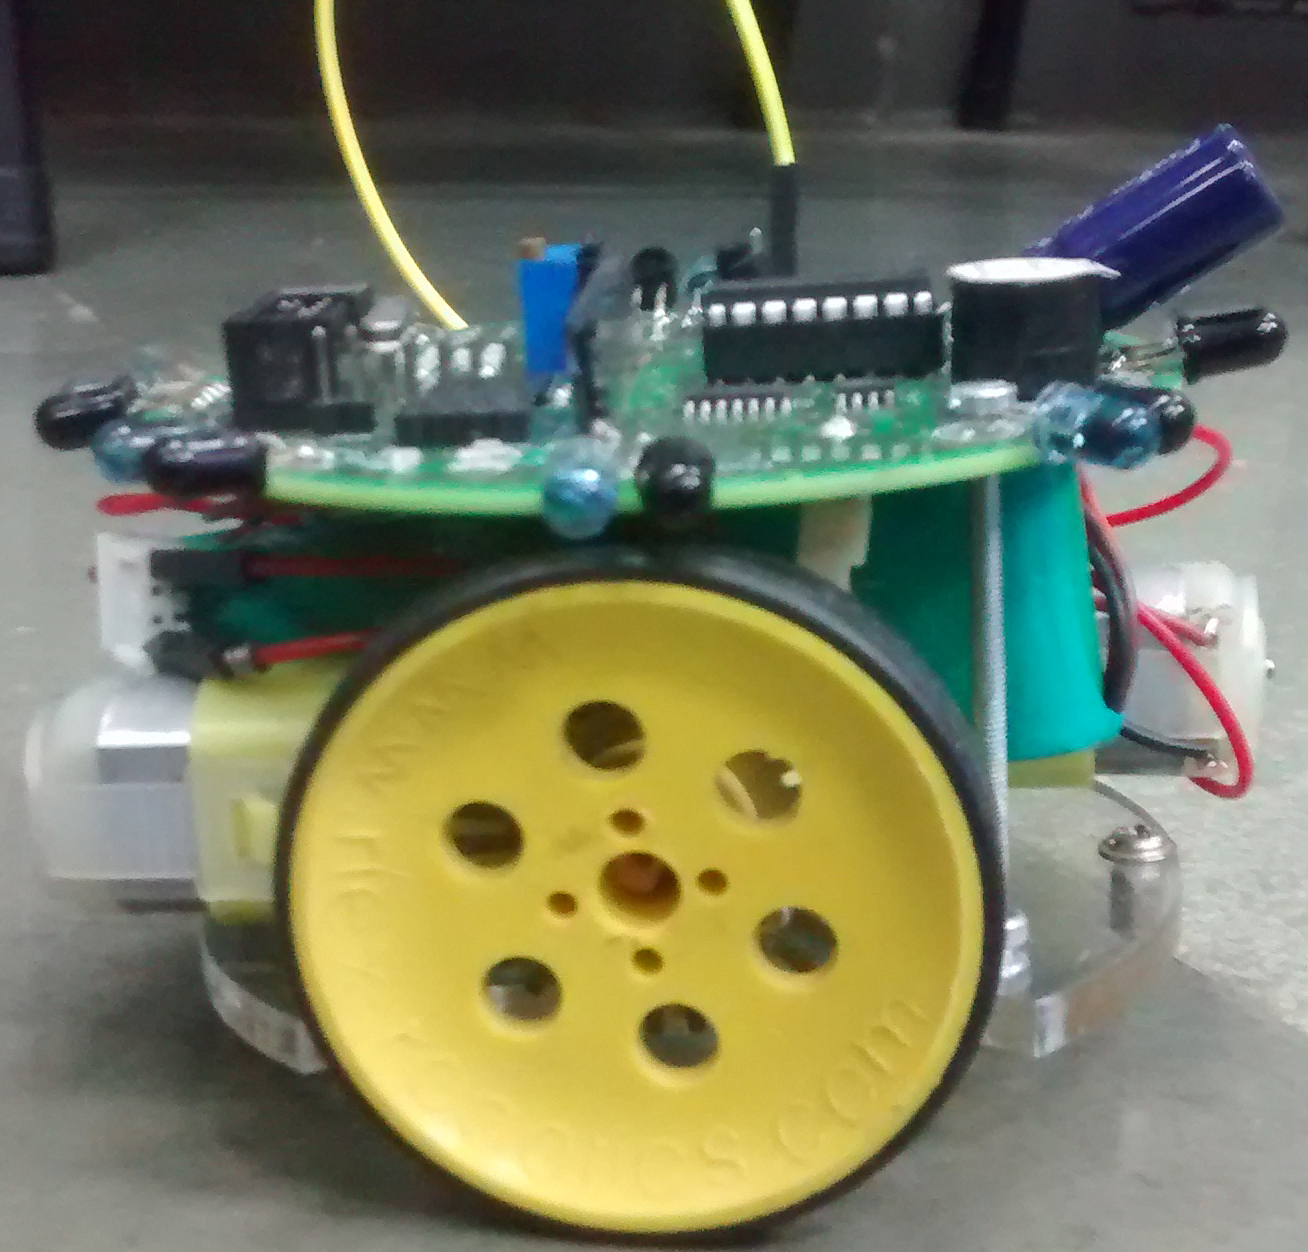
\includegraphics[width=0.30\textwidth]{./Pictures/version1_Side}
	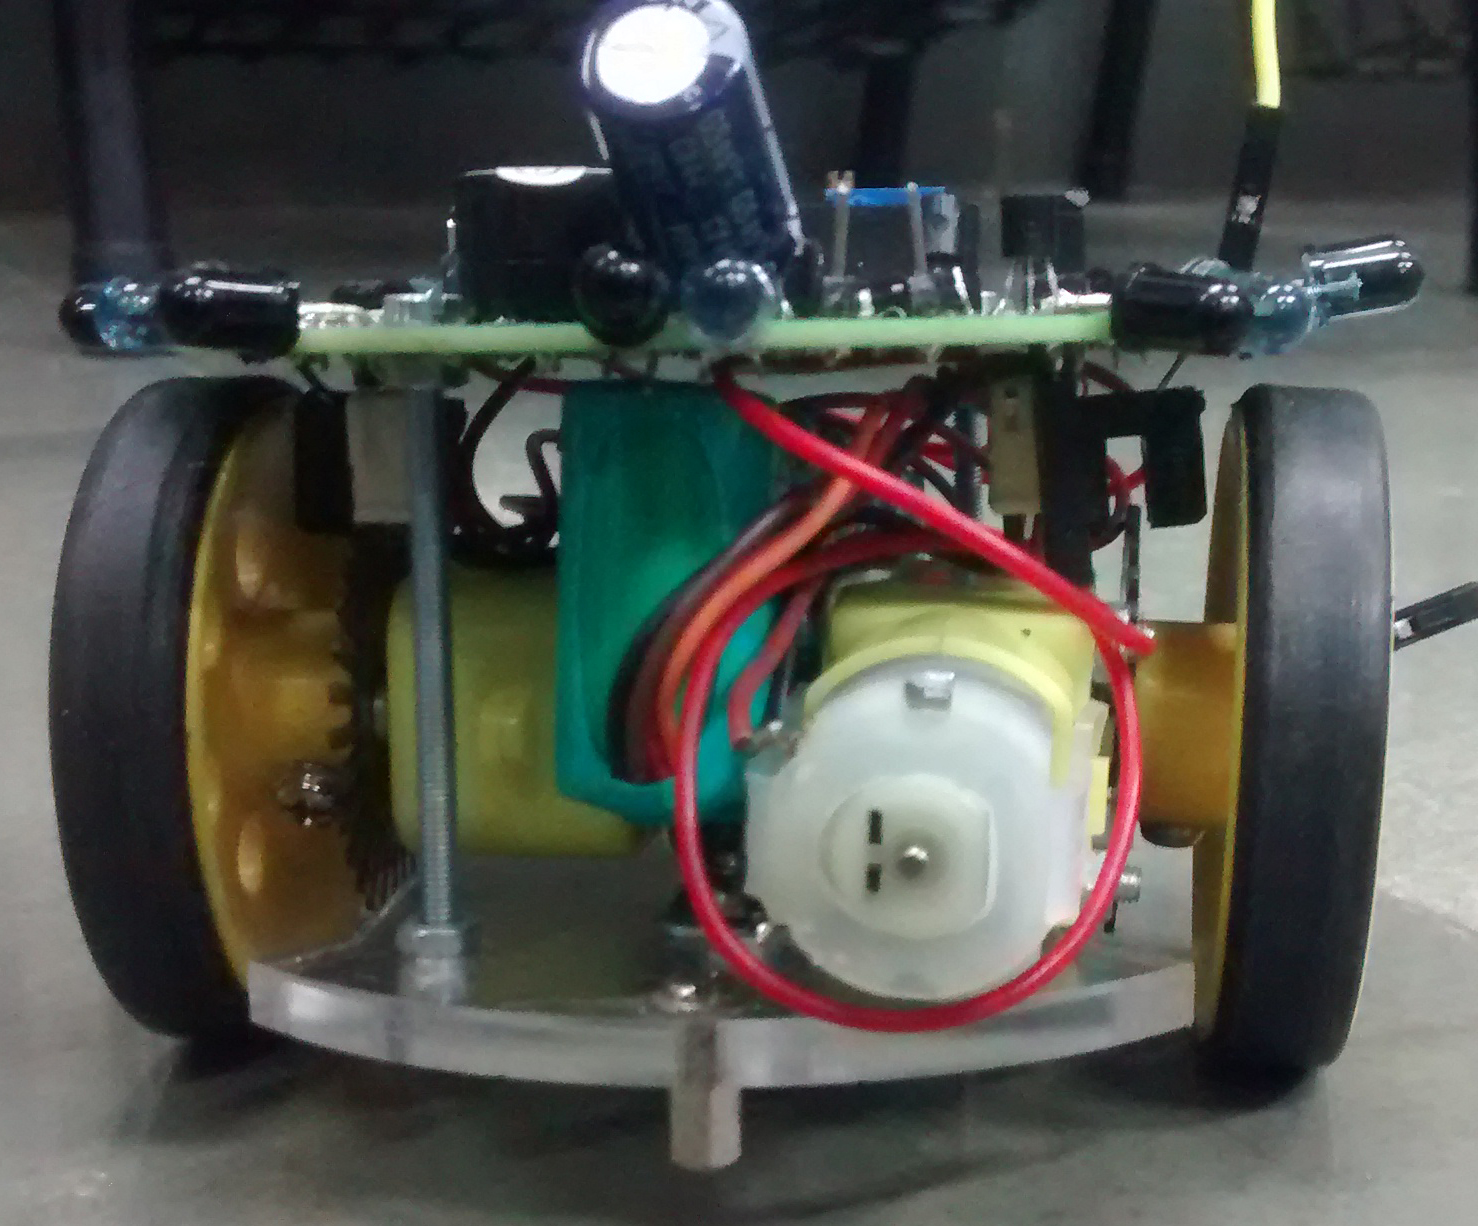
\includegraphics[width=0.30\textwidth]{./Pictures/version1_Back}
	\caption{Assembled robots}		
\end{figure}	
\hfill\\

\chapter{Software and Code}
\section{Github repository}
\href{https://github.com/eYSIP-2017/eYSIP-2017_DistributedRobotics.git}{Github link} for the repository of code

Github repository contains all the documentation and code of the project worked on. The document folder contains the manuals for hardware components/structure of Mini bots, generic shape formation algorithm for system of distributed robots and a small article to understand the working of V-REP simulator. It also contains video results of the project.

The code folder contains following codes:
\begin{itemize}
	\item C code for P controller for angular control
	\item Embedded C code for rendezvous problem (Firebird V platform)
	\item Eagle EDA project folder
	\item Test code for Mini Bots
	\item V-REP project for circle formation of fat robots
	\item V-REP project for generic shape formation
\end{itemize}

\chapter{Use and Demo}

Videos of the demos can be seen \href{https://github.com/eYSIP-2017/eYSIP-2017_DistributedRobotics/tree/master/Documents/Videos}{here}
\begin{figure}[h!]
	\centering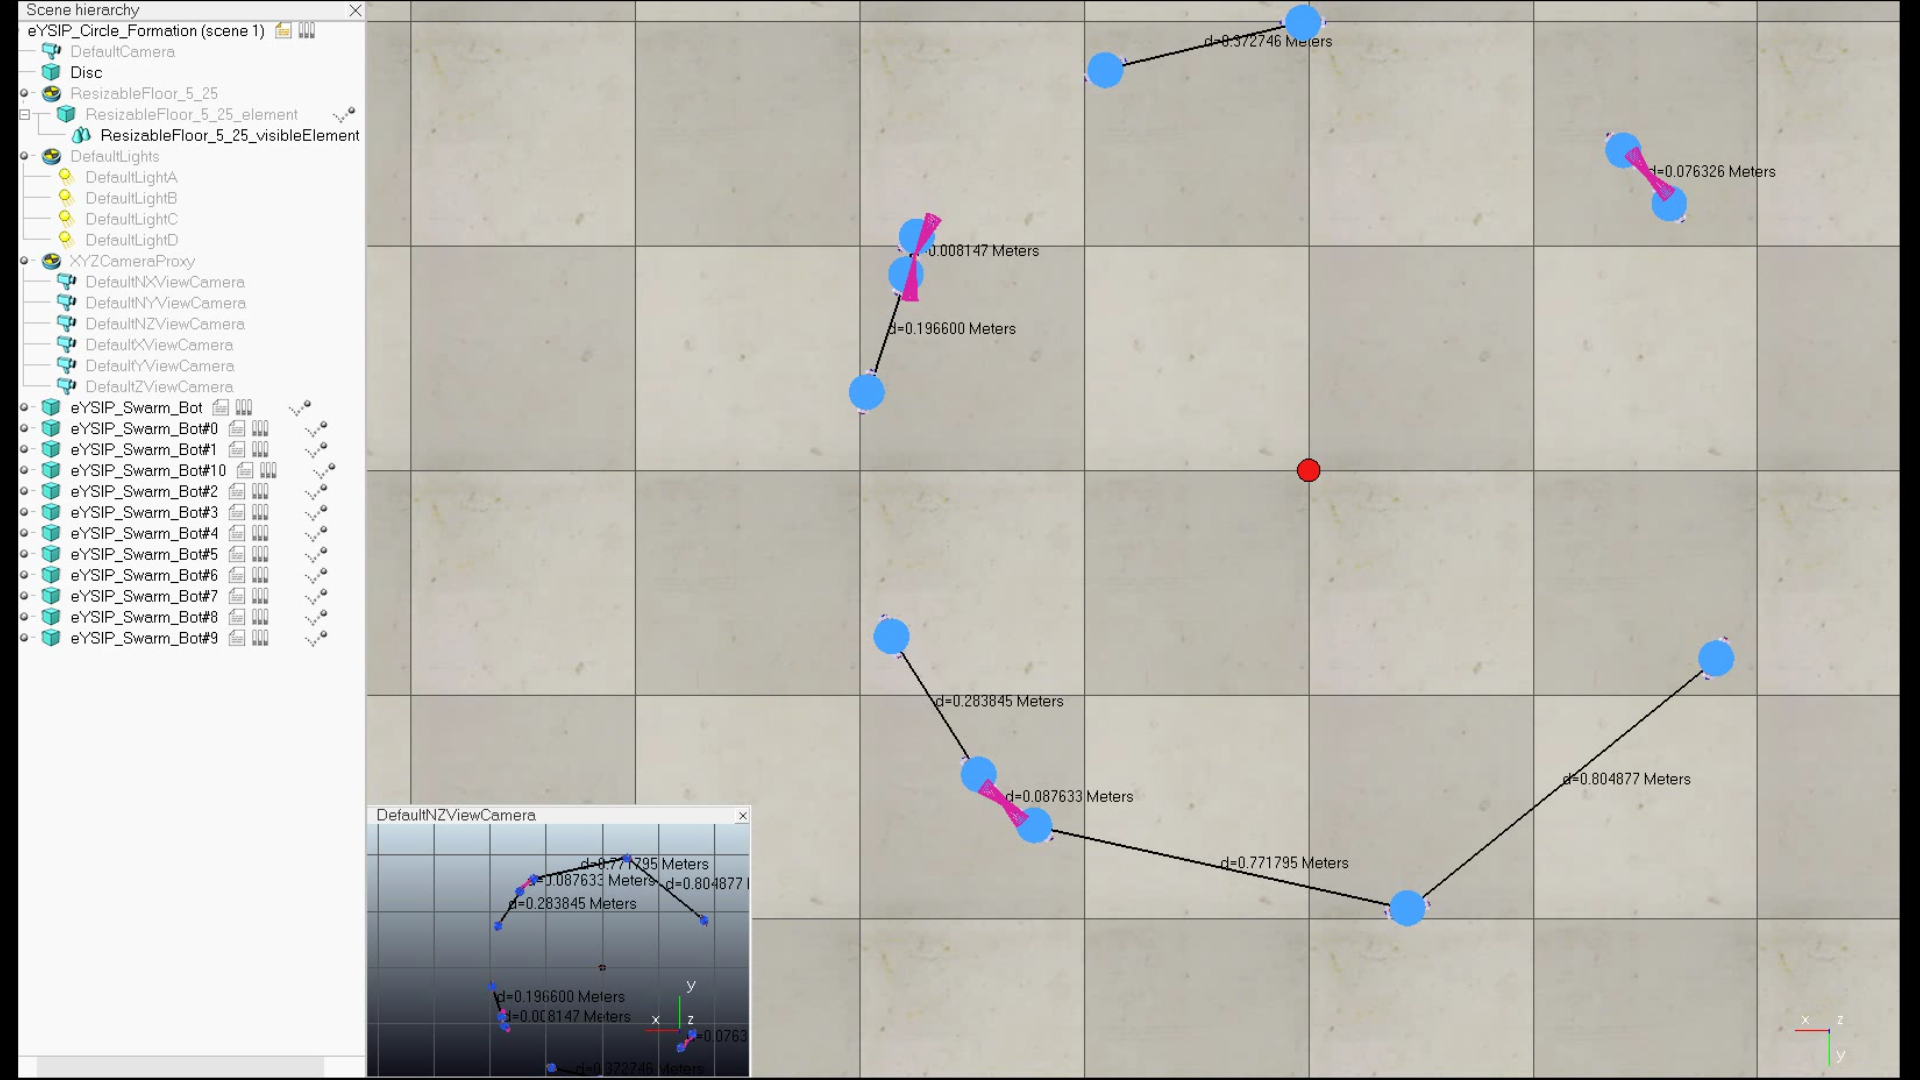
\includegraphics[width=250px]{./Pictures/Circle_formation_2}		
	\caption{Multiple robots forming a circle based on algorithm defined in "Circle formation for asynchronous fat robots with limited visibility" in V-REP simulator.}
\end{figure}

\begin{figure}[h!]
	\centering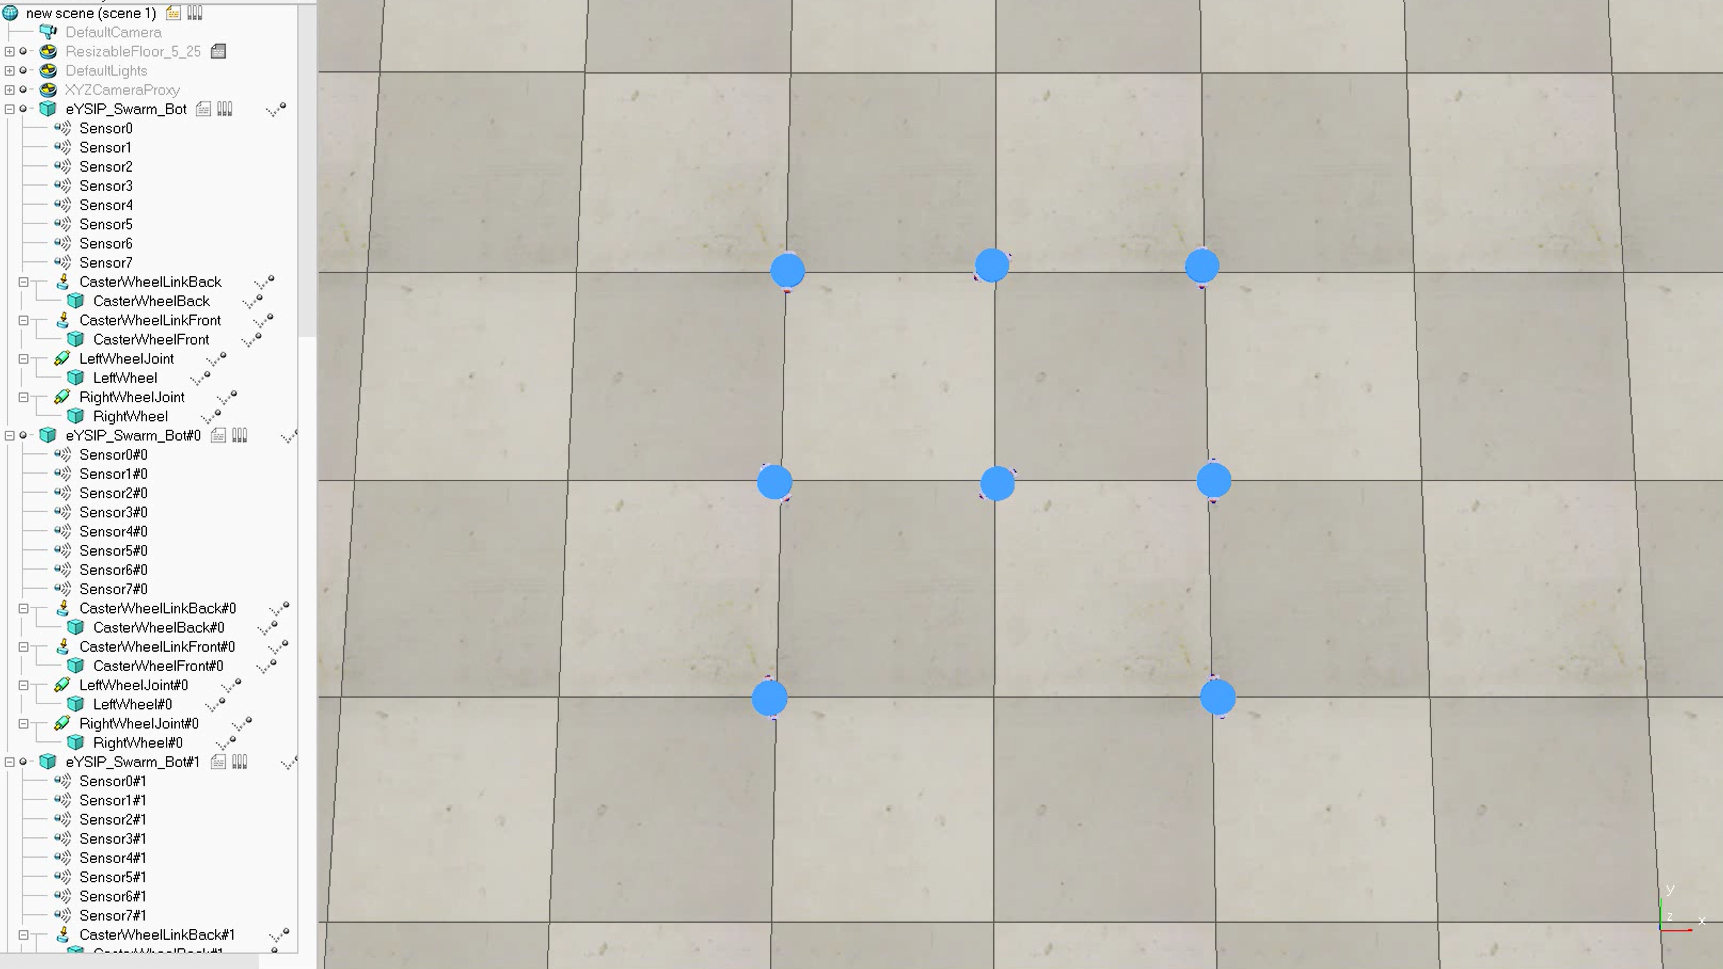
\includegraphics[width=250px]{./Pictures/A_shape}		
	\caption{Multiple robots forming shape A based on the algorithm defined in "Generic shape formation algorithm for a system of distributed robots" in V-REP simulator}
\end{figure}

\begin{figure}[h!]
	\centering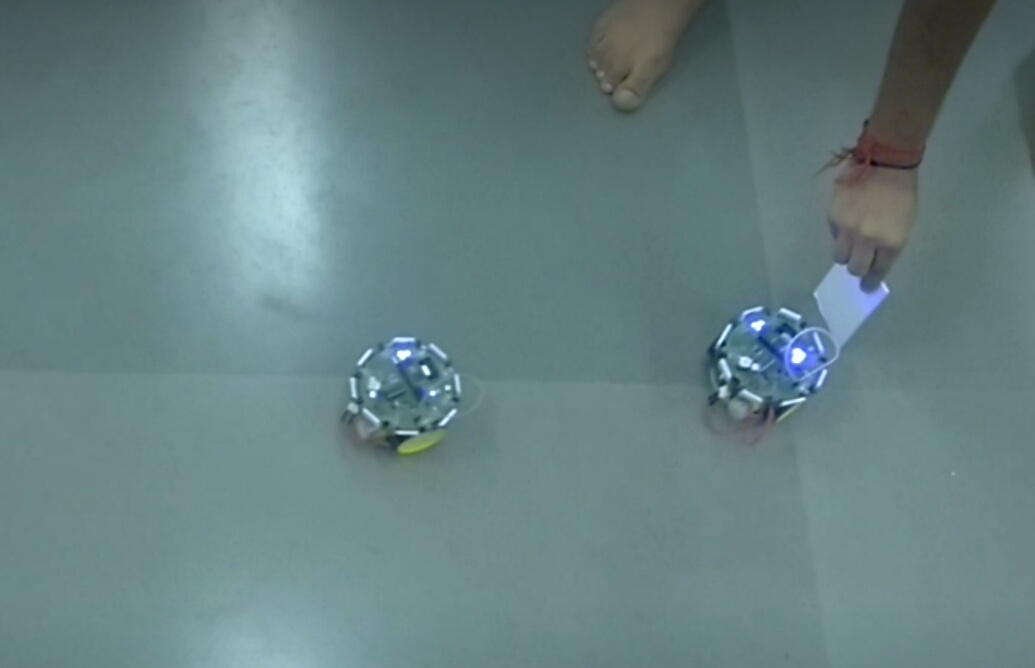
\includegraphics[width=250px]{./Pictures/Follow_lead}		
	\caption{Follow the leader swarm behavior portrayed by our Mini bots}
\end{figure}	
\newpage
\chapter{Future Work}
\begin{itemize}
	\item Design an outer covering
	\item Implementing circle formation algorithms on Mini bots
	\item Implementing gathering algorithms on Mini bots
	\item Solve shape formation with Mini Bots
	\item Solve collision of homogeneous dynamic swarm robots
	\item Find a better algorithm for tie breaking when many robots approach a single point	
\end{itemize}

\chapter{Bug report and Challenges}
\begin{figure}[h!]
	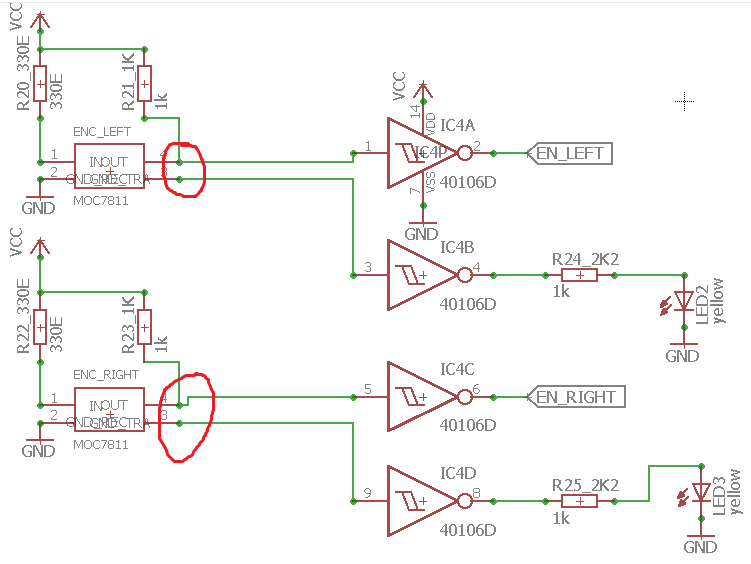
\includegraphics[width=\linewidth]{./Capture2.png}
	\caption{Position encoder connection}
\end{figure}

Bugs: Pin 3 of both encoders was supposed to be shorted to ground and connection to buffer connected to led was supposed to be shorted to pin 4\\
Fix: The bug is fixed by shorting pin 3 to ground externally\\

Challenges faced:
\begin{itemize}
	\item Placing components and routing air wires of PCB. 
	\item Reducing overall size of PCB
	\item Understanding different algorithms for circle formation and gathering algorithms for swarm robots to determine a common point for resolving global coordinate system
	\item Soldering SMD components accurately
\end{itemize}

\begin{thebibliography}{li}
\bibitem{wavelan97}
Ayan Dutta, Sruti Gan Chaudhuri, Suparno Datta and Krishnendu Mukhopadhyaya,
{\em Circle formation by asynchronous fat robots with limited visiblity}

\bibitem{wavelan97}
Sruti Gan Chaudhuri and Krishnendu Mukhopadhyaya,
{\em Gathering Asynchronous Transparent Fat Robots}

\bibitem{wavelan97}
Ayan Dutta, Sruti Gan Chaudhuri, Suparno Datta and Krishnendu Mukhopadhyaya,
{\em Circle formation by asynchronous fat robots}

\bibitem{wavelan97}
Swapnil Ghike and Krishnendu Mukhopadhyaya,
{\em A distributed algorithm for pattern formation by autonomous robots, with no agreement on coordinate compass}

\bibitem{wavelan97}
Avik Chatterjee, Sruti Gan Chaudhuri, Krishnendu Mukhopadhyaya,
{\em Gathering asynchronous swarm robots under non uniform limited visibilities}

\bibitem{wavelan97}
Krishnendu Mukhopadhyaya,
{\em Distributed swarm robotics for swarm robots}
\end{thebibliography}

\end{document}